\documentclass[../main.tex]{subfiles}

\graphicspath{{../images/}}

\begin{document}
\pagestyle{fancy}
\lhead{Lecture 3: 9/3/24}
\chead{Chapter 2}
\rhead{PHYS 421}

\section{Electrostatics}
\barh \vspace{1em}

\subsection{The Electric Field}

given charge $q$: find force on $Q$ , where $\vb F$ depends on $\boldscriptr, \vb v_i, \vb a_i$

\subsubsection{Coulombs law}

Coulomb's Law empirically,
\[\vb F_Q = \ke \frac{qQ}{\scriptr^2} \vu\scriptr\]
where $k = \frac{1}{4\pi\epsilon_0}$ and the permittivity of free space is $\epsilon_0 = \qty{8.85e-12}{C^2/Nm^2}$

\paragraph*{} The force is attractive if $sgn(qQ) = -1$ and repulsive if $= +1$.

\paragraph*{Principal of superposition:}
\begin{align*}
    \vb F_T &= \vb F_{Q1} + \vb F_{Q2} + \dots \\
    &= \ke Q \qt(\frac{q_1}{\scriptr_1^2} \vu\scriptr_1 + \frac{q_2}{\scriptr_2^2} \vu\scriptr_2 + \dots) \\
    &= Q \vb E_T
\end{align*}
where $\vb E_T$ is the total electric field due to all of the source (point) charges.

\paragraph*{}$\vb E$ doesn't depend on $Q$
\begin{itemize}
    \item $\vb E \sim F/Q$
\end{itemize}

\paragraph*{Example:} $\vb E$ field midway above two charges $q$:
\begin{figure*}[ht]
    \centering
    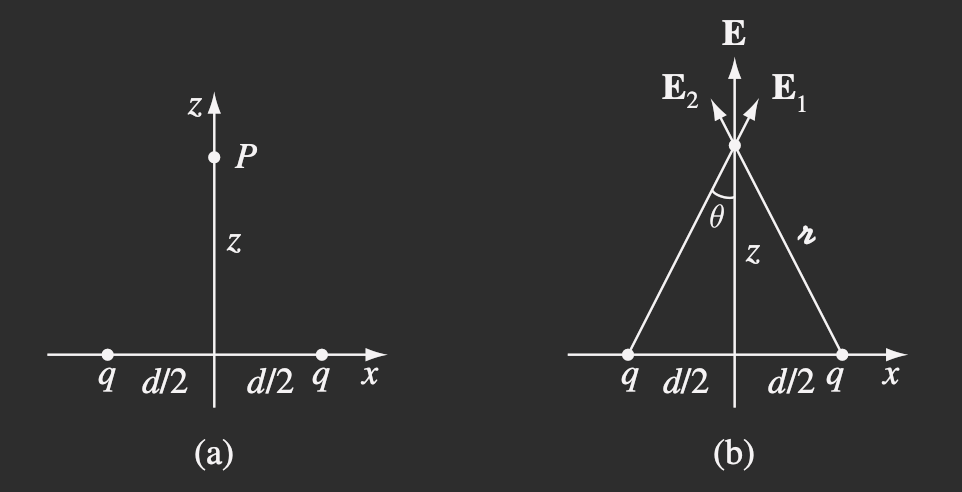
\includegraphics[width=0.5\textwidth]{ex2_1.png}
    \caption{Griffiths Example 2.1}
\end{figure*}
The electric fields are zero in the $x$ and $y$ direction:
\[E_x = E_y = 0\]
But we can sum the fields in the $z$ direction:
\[E_z = 2 \ke \frac{q}{\scriptr^2}{\cos\theta}\]
where
\[\scriptr = \qt[z^2 + \qt(\frac{d}{2})^2]^{1/2} \quad \cos\theta = \frac{z}{\scriptr}\]
so
\begin{align*}
    E_z &= \ke \frac{2qz}{\qt[z^2 + \qt(\frac{d}{2})^2]^{3/2}}
\end{align*}
Far away: $z \gg d$, so $d \to 0$ thus
\begin{align*}
    E_z &\approx \ke \frac{2qz}{z^3} = \ke \frac{2}{z^2}
\end{align*}

\paragraph*{Continuous Charge Distributions}

\begin{itemize}
    \item line: charge per unit length $\lambda; \quad \dd q = \lambda \dd \ell$
    \item surface: charge per unit area $\sigma; \quad \dd q = \sigma \dd a$
    \item volume: charge per unit volume $\rho; \quad \dd q = \rho \dd \tau$
\end{itemize}
\[\vb E(\vb r) = \ke \int \frac{1}{\scriptr^2} \vu\scriptr \dd q\]
e.g. for a volume charge:
\[\vb E(\vb r) = \ke \int \frac{\rho(\vb r')}{\scriptr^2} \vu\scriptr \dd \tau'\]
where $'$ denotes the source charge in (no $'$ is a field point)

\paragraph*{Example:} Find $\vb E$ at $z$ above a straight line segment of length $2L$ with uniform line charge $\lambda$.
\begin{figure*}[ht]
    \centering
    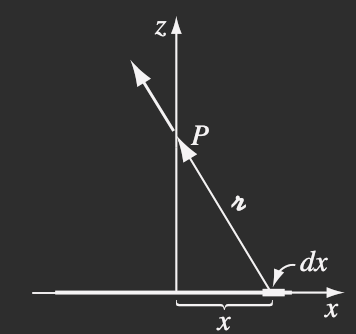
\includegraphics[width=0.3\textwidth]{ex2_2.png}
    \caption{Griffiths Example 2.2}
\end{figure*}
If we treat $\dd q$ as a point particle, then we can use Ex 2.1 likewise but integrate over the line segment. 
\paragraph*{}First we catalog what we know:
\begin{itemize}
    \item Field point $P$ is at $\vb r = z \vu z$
    \item Sources at $\vb r' = x \vu x; \quad \dd \ell' = \dd x$
    \item $\boldscriptr = \vb r - \vb r' = z \vu z - x \vu x$
    \item $\scriptr = \sqrt{x^2 + z^2}$
    \item $\vu \scriptr = \frac{\boldscriptr}{\scriptr} = \frac{z \vu z - x \vu x}{\sqrt{x^2 + z^2}}$
\end{itemize}
The electric field is then (line charge)
\begin{align*}
    \vb E(\vb r) &= \ke \int_{-L}^{+L} \frac{\lambda}{\scriptr^2} \vu\scriptr \dd x = \ke \lambda \int_{-L}^{+L} \frac{z \vu z - x \vu x}{(z^2 + x^2)^{3/2}} \dd x \\
    &= \ke \lambda \qt[z\vu z \int_{-L}^L \frac{\dd x}{(z^2 + x^2)^{3/2}} - \vu x \int_{-L}^L \frac{x \dd x}{(z^2 + x^2)^{3/2}}] \\
    &= \ke \lambda \qt[z\vu z \frac{x}{z^2 \sqrt{z^2 + x^2}}\eval_{-L}^L - \cancel{\vu x \frac{1}{\sqrt{z^2 + x^2}}\eval_{-L}^L}] \\
\end{align*}
we can easily see that the $x$ component is zero through the geometrical symmetry of the line centered at the origin (like Ex 2.1). Simplifying gives us
\[\vb E = \ke \frac{2\lambda L}{z\sqrt{z^2 + L^2}} \vu z\]
Checks and balances:
\begin{itemize}
    \item $\vu z$ is expected!
    \item \[z \gg L \quad \sqrt{z^2 + L^2} \approx z \quad E(P, z\gg L) = \ke \frac{2\lambda L}{z^2}\]
    where we can treat this as a point charge $q = 2\lambda L$ when we are far away.
\end{itemize}

\subsection{Divergence and curl of E: Gauss' Law}

`flux' of field lines
\[ \Phi = \oint_S \vb E \cdot \dd{\vb a} \]
What is $\Phi$ for point charge at origin surrounded by a spherical surface?
\begin{align*}
    \Phi &= \int \vb E \cdot \dd \vb a = \int \ke \frac{q}{r^2} \vu r \cdot \vu r r^2 \sin\theta \dd \theta \dd \phi \\
    &= \frac{q_{enc}}{\epsilon_0}
\end{align*}
\paragraph*{} A bunch of charges surrounded by a surface: \(\vb E_T = \sum \vb E_i\)
\begin{align*}
    \Phi &= \oint \vb E_T \cdot \dd\vb a = \sum_i \oint \vb E_i \cdot \dd \vb a = \sum_i \frac{q_i}{\epsilon_0}
\end{align*}
Thus we have an integral form of Gauss's law:
\begin{align*}
    \boxed{\oint \vb E \cdot \dd\vb a = \frac{Q_{\textrm{enc}}}{\epsilon_0}}
\end{align*}
where $Q = \sum q_i$.
\paragraph*{From the theorem of divergence:}
\[\oint_S \vb v \cdot \dd\vb a = \int_V (\div \vb v) \dd\tau \qand Q = \int_V \rho \dd\tau \]
so
\[\int_V (\div \vb E)\dd\tau = \int_V \rho \dd\tau \to \textrm{good for all volume}\]
therefore we have the differential form of Gauss' Law:
\[\boxed{\div \vb E = \frac{\rho}{\epsilon_0}}\]
\paragraph*{Three ways Gauss's law makes life nice: Gaussian surfaces}
\begin{itemize}
    \item spherical: gaussian sphere
    \item cylindrical: gaussian cylinder
    \item planar: gaussian pillbox
\end{itemize}

\newpage
\lhead{Lecture 4: 9/5/21}

\subsubsection{Applications of Gauss's Law}

\[\int \vb E \cdot \dd\vb a = \frac{q_{enc}}{\epsilon_0} \to \div \vb E = \frac{\rho}{\epsilon_0}\]
\begin{enumerate}
    \item (Simple spherical) What is $\vb E$ outside a uniformly charged solid sphere of radius $R$ and total charge $Q$? The spherical Gaussian surface implies a symmetry where we should \emph{only have a radial component} $\vb E = E_r$.
    \begin{align*}
        \oint \vb E \cdot \dd \vb a &= \frac{Q}{\epsilon_0} \\
        E \oint \dd \vb a = E \cdot 4\pi r^2 &= \frac{Q}{\epsilon_0} \\
        \implies \vb E &= \frac{Q}{4\pi\epsilon_0 r^2} \vu r
    \end{align*}
    where the integral is equivalent to the surface area of the sphere. This is also $\implies$ a field of a \emph{point}.
    \item (Simple cylindrical) A long cylinder (radius $a$) of charge density $\rho = ks$ ($\propto$ distance from axis) where $k$ is a constant and $s$ is the radial distance from the axis. What is $\vb E$ inside the cylinder?
    The cylindrical Gaussian surface has radius $s$ and length $\ell$:
    \begin{align*}
        \oint \vb E _\cdot \dd\vb a = \frac{Q_enc}{\epsilon_0}; \quad Q_{enc} = \int \rho \dd \tau = \int (ks') \dd s' \dd \phi \dd z = \frac{2}{3} \pi k \ell s^3
    \end{align*}
    When using the divergence theorem, note that only the curved part of the cylinder contributes to the flux. Thus,
    \begin{align*}
        \int \vb E \dd \vb a \to E\int \dd a = E (2\pi s \ell) \\
        \implies \vb E = \frac{1}{3\epsilon_0} ks^2 \vu s
    \end{align*}
    If we were to find the field outside the cylinder we would find that the enclosed charge is constant $Q_{enc}$ thus the field is proportional to $1/s$.
    \begin{figure*} [ht]
        \centering
        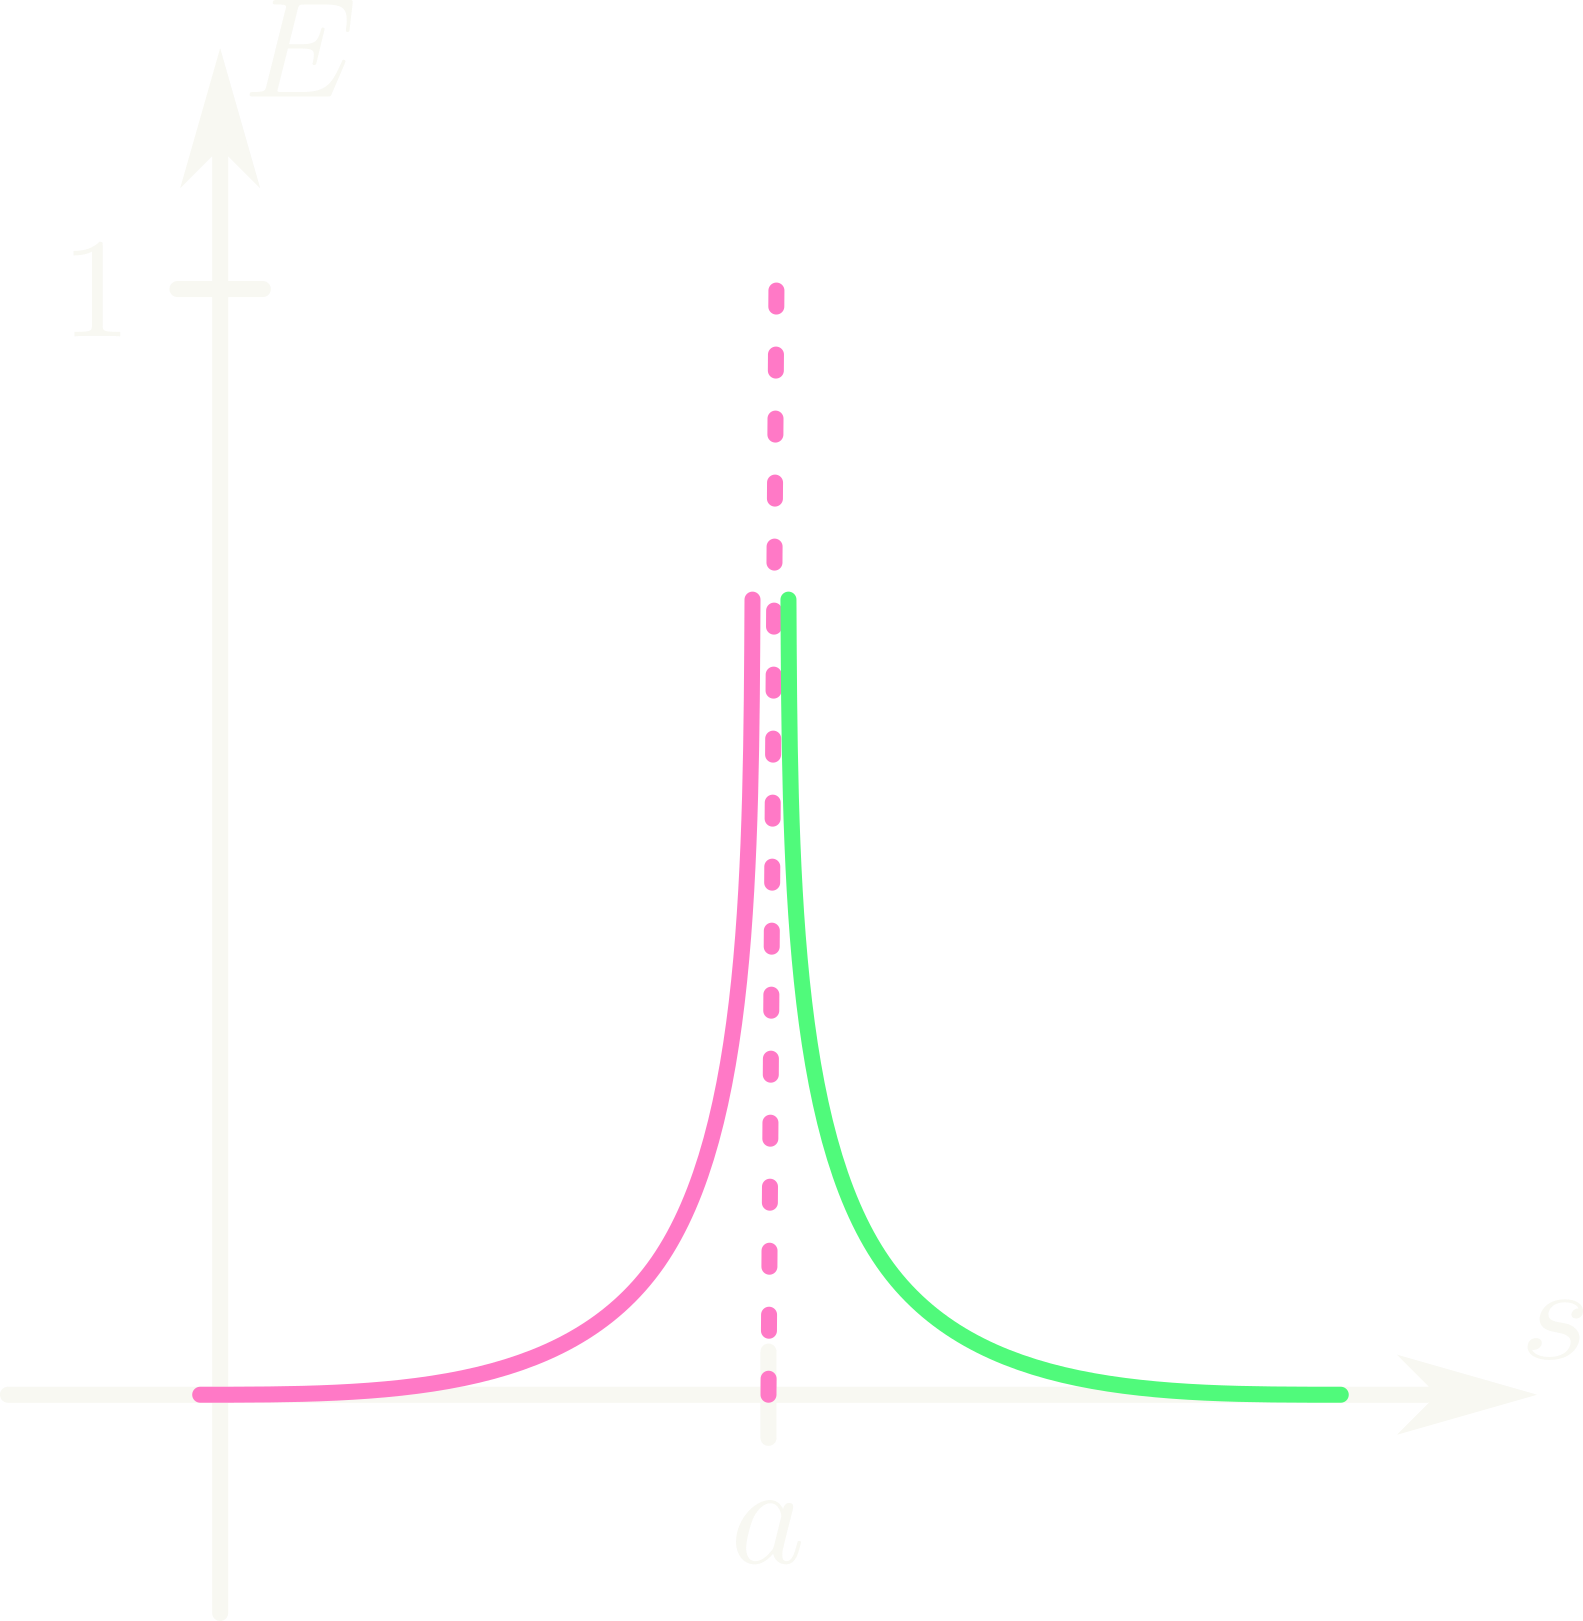
\includegraphics[width=0.3\textwidth]{fig2_3.png}
        \caption{Electric field as a function of $s$}
    \end{figure*}
    \item (Simple infinite plane) with uniform surface charge $\sigma$. Symmetry implies that $\vb E$ is perpendicular to the plane.
    The Gaussian pillbox (either box or cylinder) will have a field of
    \[\vb E = \frac{\sigma}{2\epsilon_0} \vu n \]
\end{enumerate}
\subsubsection{The curl of E}
\[\curl \vb E = 0, \quad \vb E = \frac{1}{4\pi \epsilon_0} \frac{1}{r^2} \vu r \]
calculating
\[\int_a^b \vb E \cdot \dd \ell, \quad \dd \ell = \dd r \vu r + r \dd \theta \vu*\theta + r\sin\theta \dd\phi \vu*\phi\]
So the integral is
\begin{align*}
    \ke \int_a^b \frac{q}{r^2}(\vu r \cdot \vu r) \dd r = \ke \qt(\frac{q}{a} - \frac{q}{b})
\end{align*}
This means:
\begin{itemize}
    \item path independent!
    \item if $a = b$ then $\oint \vb E \cdot \dd \vb\ell = 0$ ($\ell$ is a vector but I don't know how to bold it)
\end{itemize}
We can now use Stokes' theorem: \(\oint \vb v \cdot \dd \ell = \int_S (\curl \vb v) \cdot \dd \vb a\) or
\begin{align*}
    \oint \vb E \cdot \dd\ell = \int_S (\curl \vb E) \cdot \dd \vb a = 0 \implies \curl \vb E = 0
\end{align*}

\subsection{Electric potential}

Any function $f$ with zero curl is the gradient of a scalar function: \(\curl (\grad f) = 0\) (curl of gradient is always 0!)
\[V(\vb r) = - \int_\mathcal{O}^{\vb r} \vb E \cdot \dd \ell\]
implies all paths give some value.

\paragraph*{} $V \sim$ ``electric potential''
\begin{align*}
    V(\vb b) - V(\vb a) &= - \qt(\int_\mathcal{O}^b \vb E \cdot \dd \ell) - \qt(-\int_\mathcal{O}^a \vb E \cdot \dd\ell) \\
    &= - \int_\mathcal{O}^b - \int_\mathcal{a}{O} \vb E \cdot \dd\ell \\
    &= - \int_a^b \vb E \cdot \dd \ell
\end{align*}
And from the fundamental theorem for gradients: \(T(\vb b) - T(\vb a) = \int_a^b (\grad T) \cdot \dd\ell \)
\[\implies \vb E = -\grad V \]
\begin{enumerate}
    \item [i] ``potential'' is a terrible name
    \item [ii] $\vb E = (E_x, E_y, E_z)$ vs $V$ with only \emph{one} value at every point in space! Otherwise we would have to deal with
    \[(\curl \vb E)_x = \pdv{E_z}{y} - \pdv{E_y}{z} = 0\]
    \item [iii] \[V'(\vb r) = -\int_{O'}^{\vb r} \vb E \cdot \dd\ell = - \int_{O'}^O \vb E \cdot \dd\ell - \int_O^{\vb r} \vb E \cdot \dd\ell = C + V(\vb r) \]
    $\implies \vb E = - \grad V$
\end{enumerate}
\end{document}
